% \begin{center}
%     \begin{figure}
%         \centering
%         
\includegraphics[width=2.8cm]{Imagens/logoufpe (2).png}
%     \end{figure}   
\begin{tikzpicture}[remember picture, overlay]
    \node at (6,3.2) {
\includegraphics[width=2cm]{Imagens/logoufpe (2).png}};
\end{tikzpicture}

\begin{tikzpicture}[remember picture, overlay]
    \node at (10,3.7) {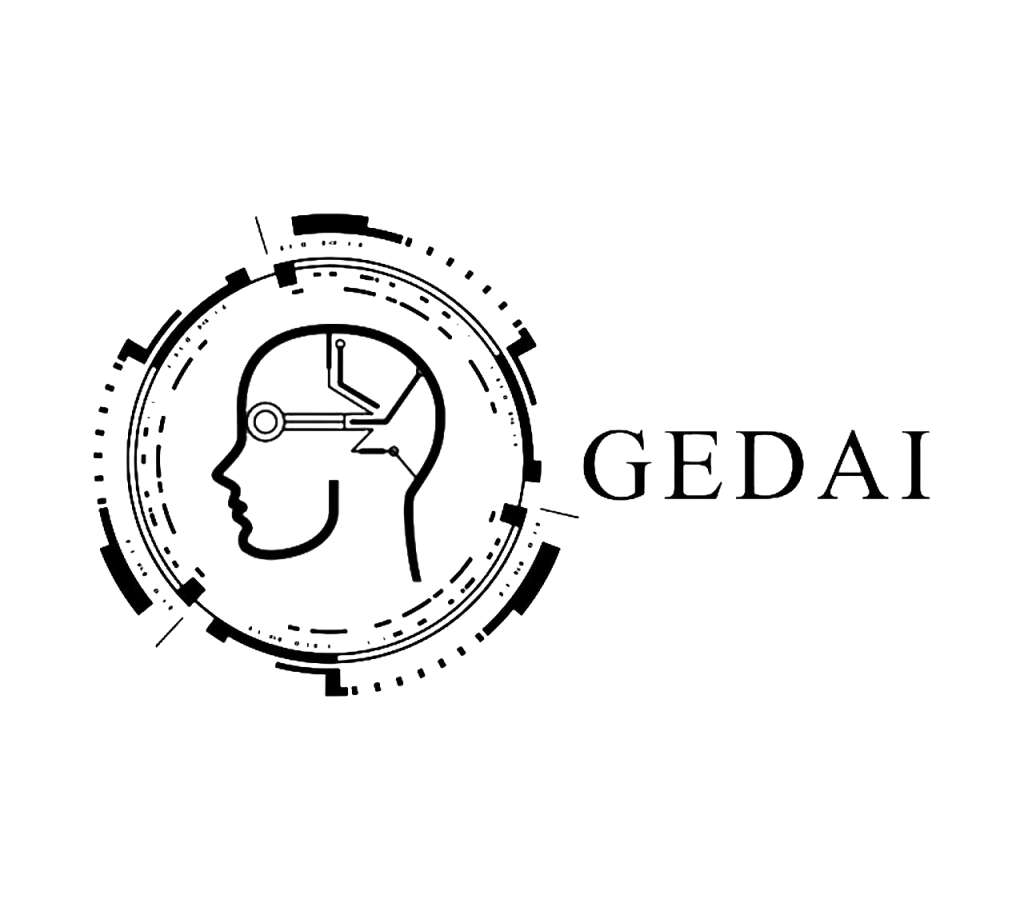
\includegraphics[width=5.5cm]{Imagens/gedai.png}};
\end{tikzpicture}



    
\begin{center}
    \tikz[baseline] {
        \node[draw=black, thick, text=white, fill=black, inner sep=5pt, rounded corners] {
            {\sffamily\bfseries\color{white} \large\textbf{RELATÓRIO DE IMPACTO DO FECHAMENTO  NA TRAVESSA 13 DE MAIO} \par}
        };
    }
\end{center}
    \vspace{2cm}
% \begin{center}  
%         UNIVERSIDADE FEDERAL DE PERNAMBUCO\\
%         CENTRO ACADÊMICO DO AGRESTE – CAA\\
%         PROGRAMA DE POS GRADUAÇÃO EM ENGENHARIA DE PRODUÇÃO\\
% \end{center}
    
        
    % \vspace{2cm}
\begin{textblock*}{10.5cm}(-0.2cm, 20cm)

\begin{tikzpicture}
    \fill[blue!80] (0,0) rectangle (10.2,7.7);
\end{tikzpicture}
\end{textblock*}

\begin{textblock*}{10.5cm}(0cm, 20cm)

\begin{center}

    
   \textcolor{white}{\textbf{Antonio Marcos De Lima}$^1$ - \href{https://orcid.org/0009-0005-5127-548X}{orcid.org/0009-0005-5127-548X} \\
    \textbf{Ronaldo Carlos da Silva}$^2$ - \href{https://orcid.org/0009-0006-0304-9151}{orcid.org/0009-0006-0304-9151} \\ 
    \textbf{Winicius A. S. Silva}$^3$ - \href{https://orcid.org/0009-0005-7934-1303}{orcid.org/0009-0005-7934-1303}\\
     \textbf{Jean Gomes Turet}$^4$ - \href{https://orcid.org/0000-0003-3608-1706}{orcid.org/0000-0003-3608-1706} \\  
    \textbf{Thyago C. C. Nepomuceno}$^5$ - \href{https://orcid.org/0000-0001-8327-6472}{orcid.org/0000-0001-8327-6472} }\\  

   
    \textcolor{white}{$^1$ Universidade Federal de Pernambuco, Caruaru, Brasil \\ Email: antonio.marcoslima@ufpe.br \\
     $^2$ Universidade Federal de Pernambuco, Caruaru, Brasil \\ Email: ronaldo.carlos@ufpe.br \\
    $^3$ Universidade Federal de Pernambuco, Caruaru, Brasil \\ Email: winicius.silva@ufpe.br \\
    $^4$ Universidade Federal de Pernambuco, Caruaru, Brasil \\ Email: jean.turet@ufpe.br\\
    $^5$ Universidade Federal de Pernambuco, Recife, Brasil \\ Email: thyago.nepomuceno@ufpe.br \\
    $^*$autores correspondentes}\\
    \vspace{0.2cm}
    \textcolor{white}{\textbf{Caruaru, 2025}}
    

\end{center}

\end{textblock*}